\documentclass[a4paper]{article}
\usepackage[T1]{fontenc}
\usepackage{amsmath}
\usepackage{hyperref}
\usepackage{amsthm}
\usepackage{amssymb}
\usepackage{float}
\usepackage{subfig}
\usepackage[utf8]{inputenc}
\usepackage[italian]{babel}
\usepackage{graphicx} 
\graphicspath{{figures/}}
\newcommand{\lcc}{\textit{largest connected component}}
\begin{document}

\author{
	Lorenzo Dentis, \textit{lorenzo.dentis@edu.unito.it}\\
	Roberto Casale, \textit{roberto.casale719@edu.unito.it}\\
	Alessandro Nocera, \textit{alessandro.nocera@edu.unito.it}
}
\title{Relazione progetto Network Science}
\maketitle

\tableofcontents


\section{Analisi}
\subsection{Dataset}
Il dataset che abbiamo analizzato è il seguente: \textit{ Friendship and Mobility: User Movement in Location-Based Social Networks }\cite{original_paper}.\\
Contiene dati anonimi estratti dal social-network \textit{Brighthike}, un social basato sulla posizione.
In qualsiasi momento un utente ha la possibilità di condividere la sua posizione e cercare altre persone geograficamente vicine che fanno uso di quel social, c'è anche la possibilità di segnalare che si è stati in un posto preciso ad una data ora.
Il dataset preso in esame è una restrizione di questi dati secondo 3 filtri:
\begin{itemize}
	\item Temporale: Sono presenti solo risultati raccolti tra Apr. 2008 e Ott. 2010.
	\item Sociale: Sono stati mantenuti solo gli archi che indicavano incontri, quindi se un nodo ha effettuato \textit{check-in} in un dato luogo ma nessuno era presente il dato è stato eliminato.
		Questo fa si che sia possibile avere archi duplicati (due persone che si incontrano diverse volte in luoghi diversi o momenti diversi) ed archi monodirezionali, ad esempio un utente potrebbe aver guardato se ci fosse qualcuno nelle vicinanze e poi non averlo contattato.\\
		Tutti gli archi monodirezionali sono stati trasformati in bidirezionali perchè per lo scopo della ricerca era importante registrare gli incontri, che questi fossero o meno rappresentativi di una interazione sociale
\end{itemize}

\subsection{Dataset e approssimazioni}
Il dataset è composto da $58228$ nodi e $214078$ archi, rappresentanti un incontro tra due nodi, ciò lo rende a volte intrattabile ma fornisce anche la possibilità di effettuare operazioni di approssimazione e vedere come queste si comportano rispetto a differenti misure.
L'operazione di approssimazione più efficace che abbiamo trovato è stata la scelta di ridurre il dataset ai soli dati raccolti in un anno (2009), ciò ha portato ad un dimezzamento dei nodi (24568 nodi e 19898 archi) rendendo possibili computazioni troppo dispendiose altrimenti.
E' stato generato anche una terzo dataset, andando a focalizzarsi sui luoghi visitati, difatti tali luoghi possono essere visti come \textit{foci} ed hanno un grosso impatto sul meccanismo di creazione degli archi.

\subsection{Distanze}
Questa è stata la prima operazione che ha richiesto una approssimazione, difatti è stato usato il grafo relativo ai dati del solo anno $2009$, dovendo cercare uno shortest path per ogni coppia di nodi l'algoritmo di \textit{path finding} verrebbe eseguito potenzialmente $n*(n-1)$, cioè $3^.363^.942^.000$. ($n$ è il numero di nodi facende parte della \textit{largest connected component}, brevemente \textit{lcc}.
Il grafo non è completamente connesso, ma un rapido controllo ha indentificato che il 96\% dei nodi si trovavano nella \lcc, quindi analizzare il grafo completo è computazionalmente troppo intensivo.


Il calcolo delle distanze sul dataset ridotto ha fornito misure in linea con quanto ci si aspettava, il diametro (il più lungo shortest path) è $16$ mentre la media è molto bassa, $1,103$. Questo valore si spiega analizzando le componenti fortemente connesse.
Vi è infatti una enorme componente connessa massimale, ma quasi tutti i nodi rimanenti sono in \textit{clusters} molto piccoli, addirittura di sole due persone. Questo abbassa tantissimo la media perciò risulta molto più interessante studiare l'\textit{average\_shortest\_path} della sola componente massimale.\\
Questi risulta essere $5,71$ in linea con l'esperimento effettuato da Stanley Milgram che rilevava 6 gradi di separazione tra tutte le coppie di nodi, in questa rete la \textit{small world hypothesis} è confermata. 

\subsection{Componenti connesse}
Analizzando tutte le componenti formtemente connesse ne individuiamo $547$, di seguito una lista delle prime 10 in ordine decrescente di dimensione.
\begin{center}\begin{tabular}{ | c | c | c | c | c | c | c | c | c | c | }
  \hline
  56739 & 49 & 11 & 11 & 10 & 10 & 9 & 8 & 8 & 7\\
  \hline
\end{tabular}\end{center}
Il 96\% dei nodi fa parte della \lcc, tutte le altre componenti connesse sono formati da meno di 3/4 nodi. 
Ci sono due differenti possibilità per spiegare questo fenomeno (le due possibilità saranno analizzate meglio nella sezione \ref{SEC:centralità}): Esiste un luogo geografico dove molte persone si sono incontrate (cioè molti utenti vivono in una area geografica ridotta) oppure esistono degli hub, degli utenti che si sposano molto ed incontrano molte persone.

\subsection{Analisi dei Degrees}
\label{SEC:Degree}
Avendo una componente connessa molto grande ed essendo questa una rete sociale ci aspettavamno una struttura \textit{core-perifery} quindi alcuni \textit{super-hubs} aventi un grado molto elevato ed una maggioranza dei nodi con un degree molto basso.
Questo è confermato dalla media dei gradi di tutti i nodi del grafo: $7.35$.
Un valore inaspettatamente basso ma che si spiega andando a verificare quanti nodi hanno pochi vicini, i nodi che hanno meno di 4 vicini sono $39586$ e quelli che ne hanno solo 1 sono $21157$, il $36\%$ dei nodi ha un solo collegamento.
Viene identificata quindi una fortissima struttura \textit{core-perifery} dove i nodi che non fanno parte del \textit{core} sono quasi completamente esclusi.
Andando ad effettuare il plot \ref{FIG:degree_dist_G} si evidenzia la distribuzione \textit{Heavy-tail} che ci aspettiamo dalle precedenti osservazioni, la maggior parte dei nodi ha un grado molto basso mentre sono pochi i nodi ad avere un grado maggiore di $10^2$.
\begin{figure*}[!ht]
\centering
\makebox[\textwidth][c]{
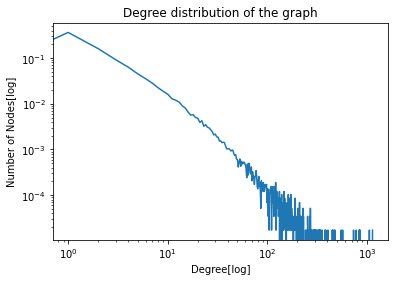
\includegraphics[width=0.85\textwidth]{degree_distribution.png}
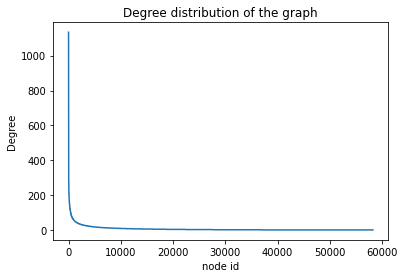
\includegraphics[width=0.85\textwidth]{nodes_degree.png}}
\caption{Degree distribution of graph} \label{FIG:degree_dist_G}
\end{figure*}
Ci sono alcui dettagli notevoli (che abbiamo notato solo dopo analisi di assortatività), in primis il numero hub è molto basso, ci sono 7 nodi che possiamo realmente definire hub (cioè nodi il cui grado è >> del grado di tutti gli altri), il secondo dettaglio è che i pochi hub hanno comunque pochi vicini.
Il massimo degree calcolato è $1134$ che è lo $0.5\%$ di tutti i link, ciò potrebbe essere dovuto al fatto che il grafo è rappresentativo di una rete sociale e quindi sparso, la conclusione è che in questa rete non ci sono hub molto grandi.
In ogni caso si nota subito che questo è un network `\textit{scale-free} in quanto segue una power-law $f(k) = k^{-c}$ con $c= 2,55$.
\subsection{Clustering coefficient e Degree correlation}
Queste due differenti analisi sono inserite nella stessa sezione in quanto hanno fornito risultati inaspettati, che hanno richiesto un'analisi più approfondita prima di essere spiegabili.
Il clusering coefficient è risultato essere $0.172$, un valore molto basso che indicava una scarsa tendenza dei nodi a rispettare la \textit{triadic clousure}.
Essendo questa una rete sociale ci aspettavamo un valore molto alto, ad indicare che se un nodo $a$ è collegato al nodo $b$ ed un nodo $c$ è collegato al nodo $a$ è molto probabile che ci sia un collegamento tra $c$ e $b$.
Alla luce di ciò abbiamo calcolato quanti triangoli del tipo $a - b - c$ fossero presenti nel grafo e ne abbiamo individuati $494728$ di cui solo $19685$ chiusi, il $3.98\%$.
La prima ipotesi per giustificare questo numero è stata la possibilità che il grafo rappresentasse un sottografo di una rete sociale, in termini semplici non è detto che le persone che un individuo frequenta online siano poi le persone con cui si incontra, è possibile che gli utenti di \textit{Brighthike} comunicassero senza incontrarsi di frequente.
Ma questa ipotesi non è molto sensata e soprattutto non è supportata da nessun dato, anzi per il fenomeno dell'affiliazione persone con \textit{foci} in comune dovrebbero tendere a formare legami sociali (il social Brighthike è un esempio di \textit{focus}).


L'ipotesi corretta, derivata dallo studio dell'assortatività e confermata dalla lettura del paper orginale, è che gli incontri tra individui non siano una forte rappresentazione della rete sociale sottostante.\\
Anche l'assortatività riporta una misura inaspettata, avendo questa un valore pari a $0.0108$ identifica che la rete non è assortativa come ci saremmo aspettati da una rete sociale, bensì neutra come un random network.
I nodi quindi non tendono a rispettare alcun criterio di assortatività, non c'è alcuna relazione tra la presenza di un arco e il grado dei nodi ai capi dello stesso.
La spiegazione di ciò la si può trovare leggendo il paper orginale: 
"We show that social relationships can explain about 10\% to 30\% of all human movement, while periodic behavior explains 50\% to 70\%"\cite{original_paper}\\
Quindi questo dataset non rappresenta perfettamente una rete sociale, pur mantenendo molte delle caretteristiche che ne definiscono una.
Essendo gli incontri tra utenti tra il 50\% ed il 70\% dovuti alla "routine" (e quindi non rappresentanti una rete sociale sottostante) molti di questi mettono randomicamente in relazione nodi che in realtà non hanno alcun legame.
\subsection{Analisi di affiliazione}
L'ultima interessante analisi svolta è stata l'analisi di affiliazione, essendo un dataset relativo a luoghi frequentati da individui l' analisi più interessante è quella dei luoghi.
I luoghi possono infatti essere visti come dei \textit{foci} ed un'analisi dei luoghi più frequentati e dei nodi che frequentano tali luoghi può fornire risultati interessanti.\\
Il risultato più interessante ottenuto è che ci sono dei luoghi dove moltissime persone si sono incontrate, il luogo più frequentato ha avuto $2606$ distinti visitatori, il $9\%$ di tutti i nodi. Il 30\% degli individui ha visitato almeno uno dei 4 luoghi più frequentati, si nota che zone corrispondono alle zone più popolose (il luogo dove si sono incontrate più persone ad esempio è il centro di Denver).

\subsection{Analisi delle comunità}
Abbiamo analizzato le comunità, in particolare abbiamo considerato solo la \lcc, dato che già sappiamo che la maggior parte dei nodi non appartenenti alla \textit{lcc} compongono \textit{clique} da 2-4 nodi disconnesse dal resto del grafo.
É stato rilevato un numero di comunità variabile tra le $150 \text{ e le } 220$, la maggior parte di piccole dimensioni (più dei 3/4 avente una dimensione massima di 100 nodi), il valore non è fisso in quanto per il calcolo è stato usato l'algoritmo di $Louvain$ che ha una assegnazione iniziale randomica.
ome mostrato in figura \ref{FIG:communities_sizes} è presente una distribuzione \textit{logaritmica} delle dimensioni della comunità.
In sintesi abbiamo poche comunità di nodi, alcune di queste molto grandi.
All'interno di queste comunità ci sono molti collegamenti, un \textit{average shortest path} molto breve che permette di attraversarle molto in fretta, e le comunità sono collegate tra loro seguendo una struttura tendente ad essere \textit{Hubs-and-spoke}, cioè esistono delle grandi comunità a cui sono connessi molte altre comunità più piccole. \\
\begin{figure*}[!ht]
\centering
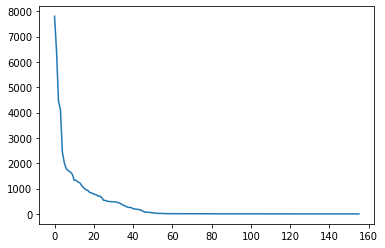
\includegraphics[width=0.7\textwidth]{community_size.png}
\caption{size of communities} \label{FIG:communities_sizes}
\end{figure*}
Tutte queste caratteristiche si osservano bene andando a costruire un grafo con le comunità come nodi.
Calcolando su questo grafo la degree correlation otteniamo un valore pari a $-0.533$ che tende ancora di più a $-1$ se consideriamo tutto il grafo e non solo la \lcc ed andando a effettuare un plot del nuovo grafo notiamo subito la struttura \textit{Hubs-and-spoke}. \\
In figura \ref{FIG:communities_plot} sono rappresentate le comunità, le etichette degli archi identificano le comunità in ordine decrescente di dimensione (0 la più grande) e il layout è basanto sull'algoritmo \textit{spring} di Fruchterman-Reingold, cioè più un nodo è distante dall'altro minori archi ci sono che collegano le due comunità.\\
\begin{figure*}[!ht]
\centering
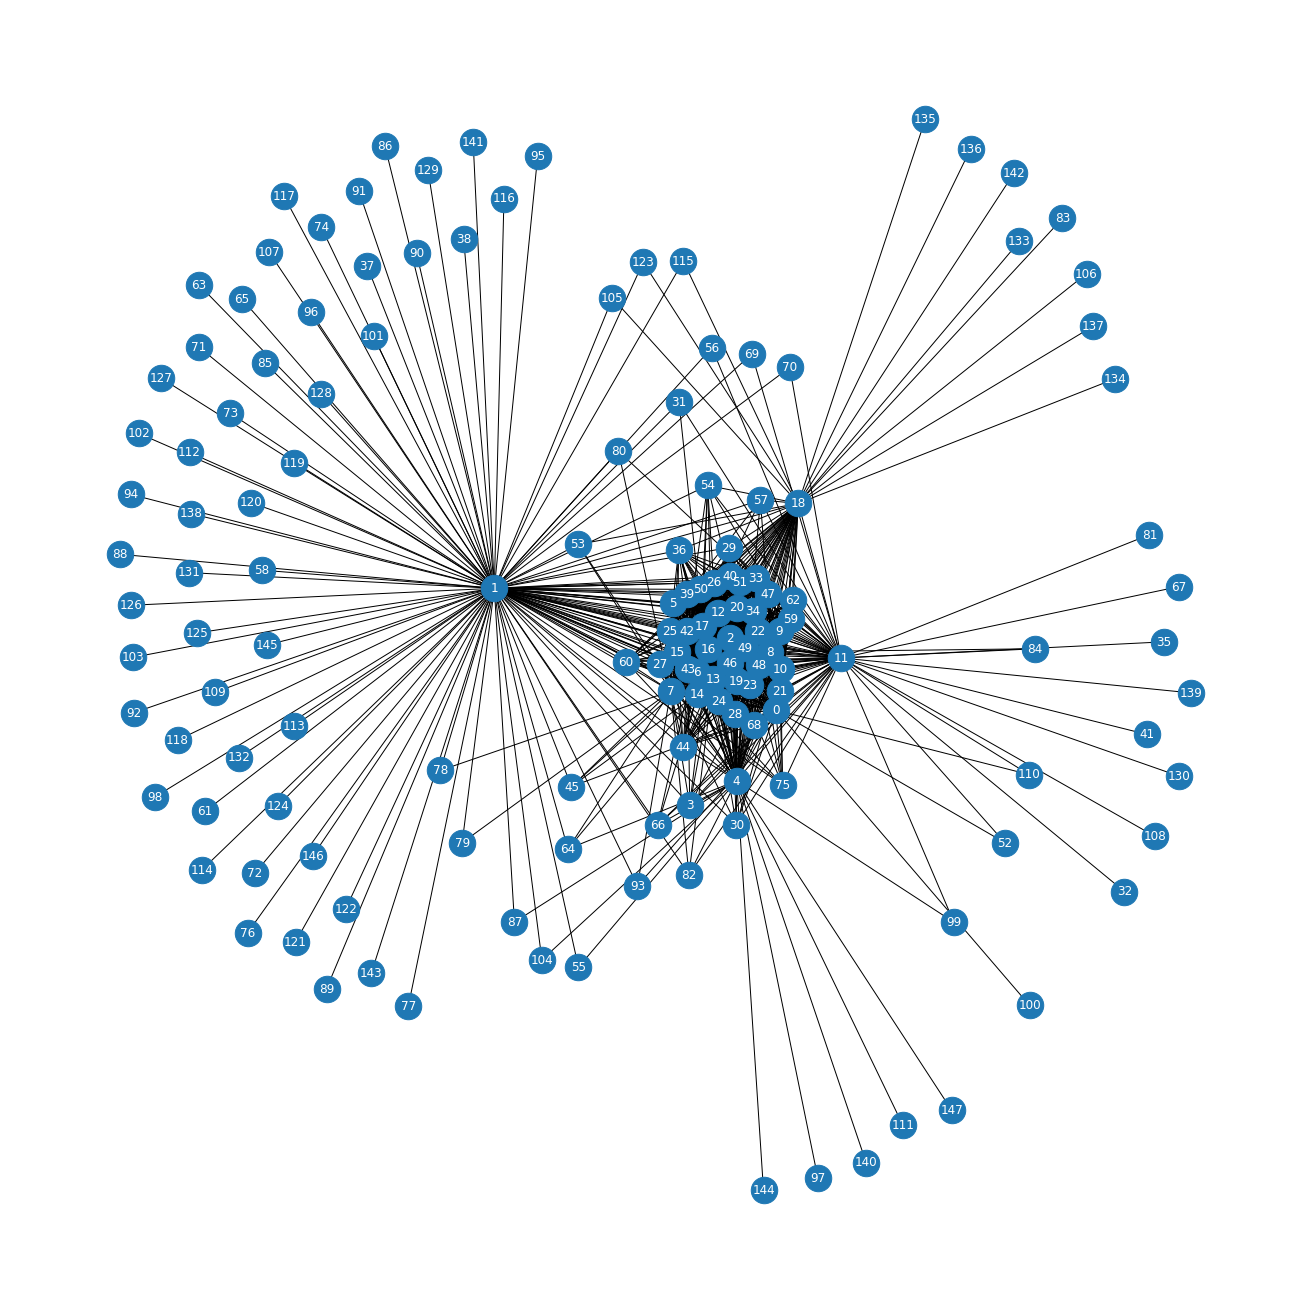
\includegraphics[width=1\textwidth]{cummunity_plot.png}
\caption{Plotting with communities as node} \label{FIG:communities_plot}
\end{figure*}
La prima cosa che si nota è che il \textit{Degree} di una comunità è proporzionale alla sua dimensione, le comunità molto grandi sono collegate a molte altre comunità (naturalmente, dato che hanno molti più componenti).\\
In secondo luogo notiamo che le comunità tendono ad essere distanti tra loro (a parte un grosso cluster in centro) ad indicare che ci sono poche connessioni inter-comunitarie.
In conclusione possiamo affermare di avere molte comunità, molto intraconnesse e poco interconnesse, c'è poi un ristretto gruppo di comunità dove l'interconnessione è molto elevata..
\subsection{Analisi di centralità}
\label{SEC:centralità}
In vista delle analisi dinamiche abbiamo appurato che sarebbe stata utile ed interessante una lista dei nodi aventi maggior \textit{betweennes}.
Il problema è che calcolare accuratamente la betweennes di un grafo con $58228$ è computazionalmente troppo intensivo, quello che abbiamo pensato di fare è stato trovare la lista di nodi a maggior \textit{degree} su un grafo ridotto e poi calcolare la betweenness approssimata sul grafo completo e confrontare i valori ottenuti per identificare eventuali variazioni.\\
\begin{figure}[!ht]
\centering
\makebox[\textwidth][c]{
	\subfloat[betweenness dei nodi a maggior degree]{\begin{tabular}{ | c | c | c | c | }
\hline
	ID & closeness & betweenness & degree\\
  \hline
40 & 0.3317& 0.1294& 1134\\
44 & 0.3008& 0.0303& 1055\\
108 & 0.3180& 0.0405& 854\\
116 & 0.3099& 0.0306& 838\\
159 & 0.3217& 0.0520& 833\\
36 & 0.3145& 0.0434& 779\\
191 & 0.3237& 0.0621& 732\\
49 & 0.3043& 0.0130& 569\\
634 & 0.2747& 0.0106& 550\\
156 & 0.2966& 0.0066& 475\\
35 & 0.3106& 0.0249& 467\\
  \hline
\end{tabular}}
\qquad
\subfloat[degree dei nodi a maggior betweenness]{\begin{tabular}{ | c | c | c | c | }
\hline
	ID & closeness & betweenness & degree\\
  \hline
40 & 0.3317& 0.1201& 1134\\
191 & 0.3237& 0.0695& 732\\
159 & 0.3212& 0.0562& 833\\
44 & 0.3008& 0.0510& 1055\\
108 & 0.3181& 0.0451& 854\\
36 & 0.3145& 0.0387& 779\\
116 & 0.3095& 0.0386& 838\\
35 & 0.3106& 0.0227& 467\\
49 & 0.3043& 0.0176& 569\\
1100 & 0.3018& 0.0168& 333\\
212 & 0.3010& 0.0158& 327\\
  \hline
\end{tabular}}}
\end{figure}
Ciò che abbiamo individuato è che nel nostro grafo la betweenness non è necessariamente legata al grado di un nodo,ci sono nodi aventi betweenness molto altra pur avendo un grado non massimo, questi sono i $broker$ che fungono da collegamento tra le varie comunità, soprattutto tra le comunità più grosse 
Però in linea di massima possiamo assumere che un nodo avente un grado alto avrà una betweenness quantomento considerevole, se non elevata (gli unici casi aventi grado non alto (non si può definire 333 basso) e betweenness alta sono il nodo 1100 ed il nodo 212).

%TODO: che altre analisi si possono fare?
\section{Simulazione dinamica}
Avendo tra le mani un dataset che riportava spostamenti ed incontri tra individui l'analisi dinamica più interessante (anche se purtroppo la più ovvia) è quella di lanciare una simulazione epidemica.
È stato utilizzato un modello SIR con i seguenti parametri:
\begin{align*}
\tau = 0.056\\
\gamma = 0.045\\
\end{align*}
Questi valori non sono casuali bensì sono valori ottenuti dallo studio del COVID-19, in particolare estrapolati dallo studio \textit{Estimation of SIR model’s parameters of COVID-19 in Algeria} \cite{covid}.
È stato scelto proprio il COVID-19 perchè è molto attuale; il lato negativo di questa scelta è che è scontata e poco creativa, quello positivo è che ci sono moltissimi studi in merito e moltissimi dati.


Sono state lanciate diverse simulazioni epidemiche andando a variare il numero di "pazienti 0" e le loro caratteristiche.
In modo da studiare come la rete interagisce con la diffusione, non sono mai stati modificati i valori di $\tau$ e $\gamma$.\\

\subsection{Pochi infetti, casuali}
La prima serie di run è stata effettuata con pochi infetti iniziali, 5 individui, il grafico in figura \ref{FIG:generic} mostra l'andamento di $S, R, I$ in relazione al tempo.
La media delle persone infettate è stata di $32.578$ individui che in un momento o in un'altro hanno contratto l'infezione nell'arco di 250 giorni, il 55\% della popolazione.\\
\begin{figure*}[!ht]
\centering
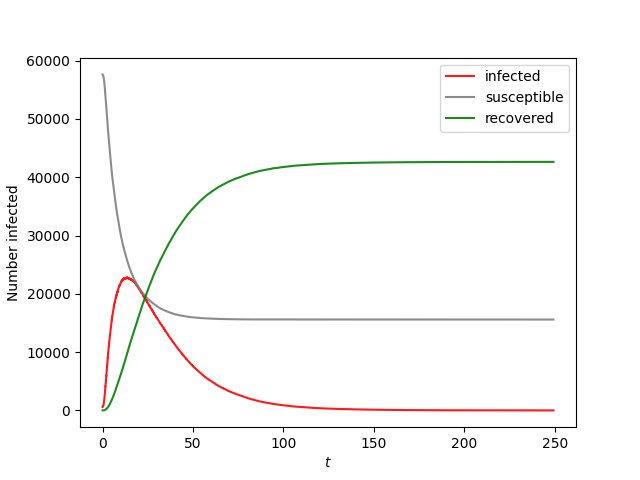
\includegraphics[width=0.8\textwidth]{generic_run.png}
\caption{Generic contagion} \label{FIG:generic}
\end{figure*}

Per dare un po' di contesto si fa notare che in 2 anni il numero di casi di COVID-19 in italia ha coinvolto il 33\% della popolazione.
Questo valore molto alto è dovuto in parte ai parametri impostati (ad esempio $\gamma$ molto basso) ma soprattutto alla forte connessione nel grafo.
Infatti una stima di $R_0$ fornisce un valore elevatissimo, pari a $34.367$, questo a causa dell'elevato numero di vicini che alcuni nodi hanno.
Se è infatti vero che (come affermato in sezione \ref{SEC:Degree}) la maggior parte dei nodi ha pochi vicini è anche vero che ci sono comunque tanti nodi aventi $Degree$ elevati.
Perciò si verifica rapidamente un effetto cascata che però notiamo si arresta prima di aver infettato tutti i nodi del grafo, infatti in media $25650$ individui non sono mai stati infettati.
Questo si spiega di nuovo ragionando sui $Degree$ dei nodi, come detto in precendenza ci sono moltissimi nodi con pochi vicini.
Perdipiù dall'analisi del grafo abbiamo individuato un forte numero di comunità molto separate tra loro, la nostra ipotesi è che si verifichi un fenomeno simile a quello del $\lambda - clustering$ che impedisce all'epidemia di penetrare in alcune comunità rendendo difficoltosa l'infezione di tutto il network.

\subsection{Variazione numero e tipo di infetti iniziali}
Per analizzare il comportamento dell'infezione sulla rete abbiamo provato a studiare i diversi "pazienti 0" da cui l'infezione può partire.
Grazie alle analisi effettuate nella sezione \ref{SEC:centralità} sappiamo che i nodi con massima \textit{betwennes} non sono quelli con \textit{degree} più elevati, ma ci aspettiamo che questi causino un effetto cascata più significatico e che i nodi con maggior \textit{betweennes} causino un contagio più diffuso.

Perciò il primo tentativo fatto è stato lanciare l'infezione con un solo paziente 0, scelto randomicamente.\\
\begin{centering}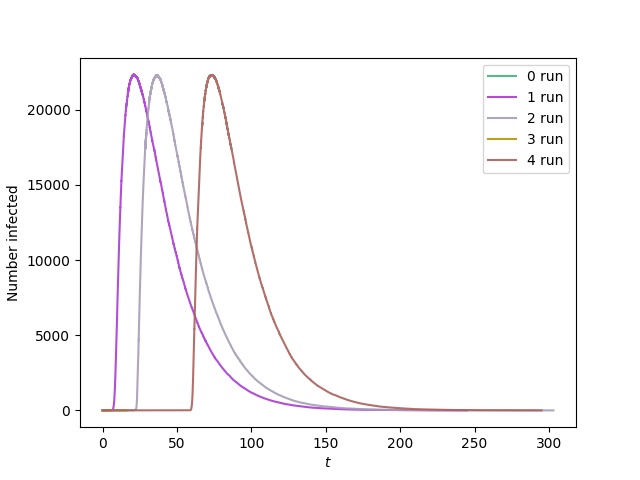
\includegraphics[width=1\textwidth]{1_random.png}\end{centering}\\
A seconda della tipo di paziente scelto abbiamo avuto risultati differenti.
\begin{itemize}
	\item La run numero 1 presenta un paziente probabilmente di grado o betweenness elevata, infatti si verifica quasi subito un effetto cascata.
	\item La run numero 4 presenta una grossa fase di "quiescenza" prima dell'effetto cascata, il paziente probabilmente apparteneva a un piccola comunità che poi ha infettato la comunità più grande.
	\item La run numero 2 presenta una situazione intermedia tra le due descritte prima
	\item Le run numero 0 e 3 non hanno creato alcuna epidemia, i pazienti 0 appartenevano ad una comunità piccola e segregata o erano addirittura fuori dalla largest component.
\end{itemize}
Basandoci su questi risultati abbiamo continuato lo studio facendo partire l'epidemia dai peggiori candidati, un nodo con minor degree e 10 nodi con degree minimo\\
\begin{figure*}[!ht]
\centering
\makebox[\textwidth][c]{	
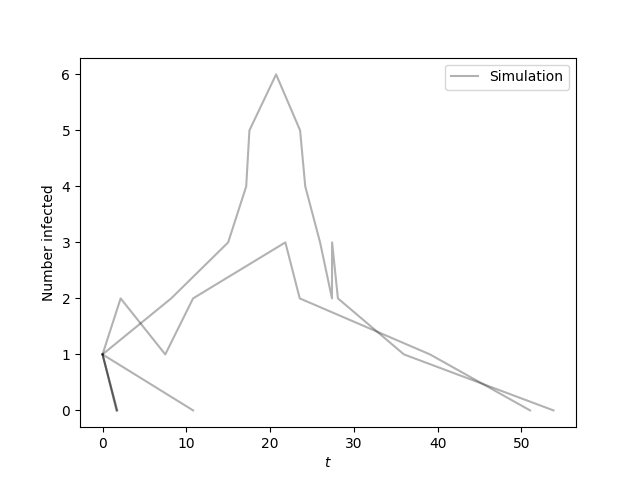
\includegraphics[width=0.85\textwidth]{1_worst.png}
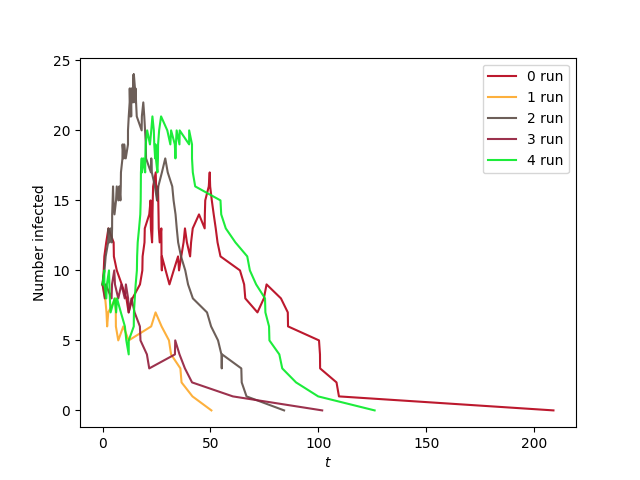
\includegraphics[width=0.85\textwidth]{10_worst.png}}
\caption{1 paziente (5 run) vs 10 pazienti} \label{FIG:bad_diffusion}
\end{figure*}\\
In questo caso non si verifica alcun effetto cascata.I pazienti iniziali appartenevano tutti a piccole comunità probabilmente (ricordo che ci sono molte comunità dense ma poco interconnesse) ed il contagio non si è diffuso abbastanza velocemente per generare un effetto cascata. Notiamo in particolare nel grafo di sinistra 3 run (tutte grigie) in cui il paziente non ha infettato nessuno ed è semplicemente guarito, questo perchè non è riuscito ad infettare il suo unico vicino.
\newline \newline
Se invece i pazienti iniziali sono nodi con molti vicini (quindi presumibilmente hanno una betweenness elevata) la situazione è molto differente.
Questo è il grafico di sviluppo epidemico con i 10 nodi aventi grado più elevato come pazienti iniziali.\\
\begin{centering}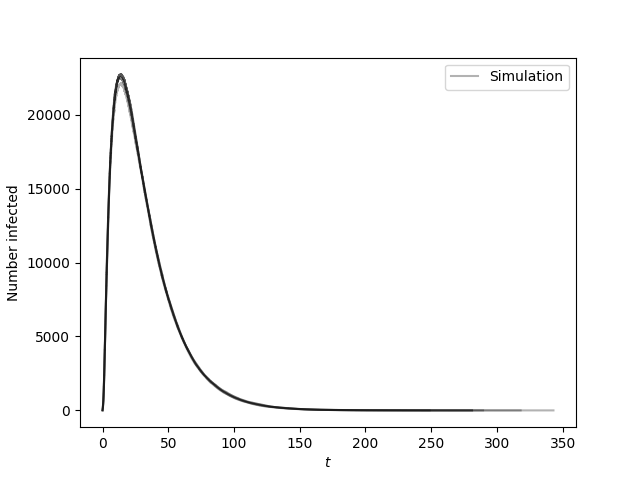
\includegraphics[width=1\textwidth]{10_best.png}\end{centering}\\
mentre questo è lo sviluppo epidemico utilizzando come paziente 0 il nodo che ha il degree più alto (questo nodo in particolare ha anche la betweenness massima).
\begin{centering}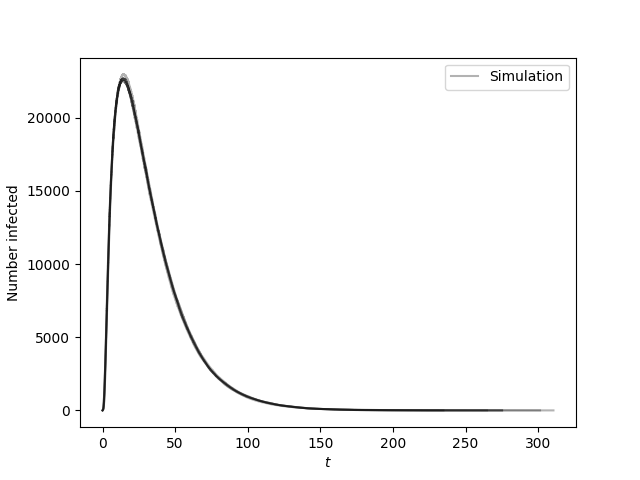
\includegraphics[width=1\textwidth]{1_best.png}\end{centering}\\
Come si può notare in tutte le run si è verificato un contagio di più di 20000 individui ed un effetto cascata quasi istantaneo, questo partendo da un solo paziente iniziale.
Come anche affermato a lezione l'infezione di un hub ha effetti molto importanti sullo sviluppo dell'epidemia, così come la struttura del grafo.


\subsection{Transmission rate}
$R_0 = 34$ è un valore molto alto, andando ad abbassare questo valore (ad esempio modificando il parametro $\tau$) si ottiene una curva epidemica più moderata.
Il grafico in figura \ref{FIG:transmission_rate_06_1_random} mostra la diffusione impostando $\tau = 0.006$ ed ottenendo $R_0$ vicino a 1.\\
\begin{figure*}[!ht]
\centering
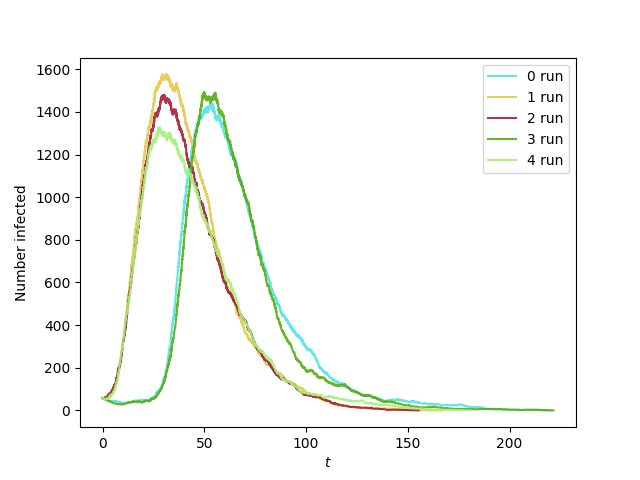
\includegraphics[width=0.7\textwidth]{transmission_rate_06_1_random.png}
\caption{Lower $R_0$} \label{FIG:transmission_rate_06_1_random}
\end{figure*}\\
Si nota una trasmissione molto ridotta ed un numero di infetti molto inferiore, ma C'è anche da considerare che un parametro di infezione così basso è irrealistico, vorrebbe dire infettare 1 individuo su 600 incontrati.


\newpage
\section{Random Models}
In questa sezione del progetto tratteremo le analisi che sono state condotte su alcuni modelli per la creazione di grafi randomici e come questi ultimi differiscano dal nostro grafo.
I modelli considerati sono:
\begin{itemize}
	\item Erdos-Renyi.
	\item Watts-Strogatz
	\item Barabasi-Albert
\end{itemize}
Altri modelli, quali: Configuration	model e Stochastic bloc model non sono stati considerati poichè i risultati ottenuti erano poco interessanti o rilevanti.

\subsection{Erdos-Renyi}
In questo tipo di modello è possibile modificare il numero di nodi e la probabilità con la quale essi si andranno a collegare. Osservando i dati ottenuti, cambiando il numero di nodi ma lasciando la probabilità invariata si riscontra una proporzione tra il numero di nodi e gli archi creati. Quello che otteniamo sempre sono grafi composti da una largest connected component costituita da tutti i nodi disponibili, un altro aspetto che risalta è il grado medio dei nodi che nonostante una probabilità bassa (es.: 0,2) rimane alto, ovviamente più aumentiamo la probabilità più aumenta il grado medio. Questo dato possiamo metterlo in relazione con quello ottenuto dal nostro grafo di partenza che risulta avere un grado medio dei nodi molto basso per via della presenza di molti nodi fuori dalla largest connected component.
Altri dati che risaltano sono la Degree Correlation che risulta essere sempre in un intorno dello zero. Questa situazione l’abbiamo anche riscontrata nel nostro grafo.
Un altro dato interessante è il Clustering Coefficent, poiché nei grafi randomici che otteniamo più aumentiamo la probabilità più il dato cresce e viceversa, mentre nel nostro grafo di partenza questo valoro è molto basso. Quindi in generale i grafi che otteniamo non sono grafi bipartiti.
Infine, un altro dato che spicca è la Betweeness Centrality che nei grafi randomici ottenuti risulta essere in generale molto bassa quindi i grafi ottenuti non presentano nodi hub o coppie di nodi che costituiscono ponti.


\subsection{Watts-Strogatz}
In questo modello invece è possibile andare a modificare il numero di nodi, il grado iniziale dei nodi e la probabilità che i collegamenti iniziali vengano ricablati. In generale i grafi che otteniamo sono pressocché identici, ovvero grafi con un unico largest connected componnet formato da tutti i nodi disponibili, un Clustering Coefficent basso (da 0,15 a 0,3), una Degree Correlation neutra e una Betweeness Centrality veramente molto bassa, quindi grafi tendenzialmente bipartiti e senza hubs o bridge. Nel caso in cui però dovessimo aumentare il valore della probabilità il valore che presenta una diminuzione notevole è quello del Clustering Coefficent, che può arrivare anche a uno 0,02. Un altro caso interessante è il caso in cui diminuiamo considerevolmente il valore del secondo parametro (grado iniziale dei nodi), andando a modificare questo parametro, otteniamo grafi con più Largest connected component (anche se vi è sempre una di maggiore dimensione rispetto alle altre).
Quindi in generale quello che otteniamo sono grafi dissimili dal nostro fatta eccezione per il valore della Degree Correlation.



\subsection{Barabasi-Albert}
In questo modello posso modificare: il numero di nodi del mio grafo e il numero di archi da creare da un nuovo nodo ai nodi preesistenti.
I vari grafi che otteniamo sono grafi con valori di Betweeness Centrality molto bassi e una Degree Correlation sempre nell’intorno dello zero quindi non possiamo capire se il grafo è assortativo o no. Nel caso in cui dovessi aumentare notevolmente il numero di archi da creare da un nuovo nodo ai nodi preesistenti, il valore di Clustering Coefficent aumenterebbe; quindi, ottengo dei grafi che sono simili a dei social network. In conclusione, i grafi che otteniamo sono diversi dal grafo di partenza tranne per il valore della Degree Correlation.
\begin{thebibliography}{9}

\bibitem{original_paper}
E. Cho, S. A. Myers, J. Leskovec (2011) \emph{Friendship and Mobility: User Movement in Location-Based Social Networks}\\
CM SIGKDD International Conference on Knowledge Discovery and Data Mining (KDD)\\
\href{http://snap.stanford.edu/data/loc-brightkite.html}{Link to dataset}\\
\href{https://cs.stanford.edu/people/jure/pubs/mobile-kdd11.pdf}{Link to paper}

\bibitem{covid}
Mohamed Lounis and Dilip Kumar Bagal (2020) \emph{Estimation of SIR model’s parameters of COVID-19 in Algeria}\\
Bull Natl Res Cent PMCID: PMC7570398
\href{https://www.ncbi.nlm.nih.gov/pmc/articles/PMC7570398/}{Link to study}
\end{thebibliography}

\end{document}

